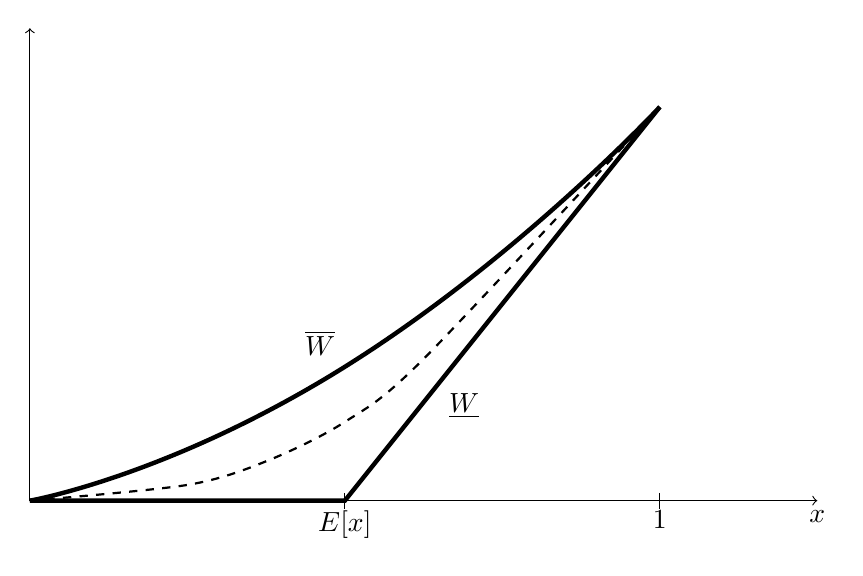
\begin{tikzpicture}[xscale=1,yscale=1] 

		\draw [<->] (0,6) 
		        |- (10,0) node (xaxis) [below] {$x$};
	
	%\draw[step=1cm,gray,very thin] (0,0) grid (10,6);


	\draw[ultra thick] (0,0) -- (4,0) -- (8,5); 
	\node at (5.2,1.2)[right] {$\underline W$};


	\draw[ultra thick] plot [smooth,tension=1] coordinates {(0,0) (4,1.7) (8,5)};
	\node at (4,2)[left] {$\overline W$};


	\draw[thick,dashed] plot [smooth,tension=.5] coordinates {(0,0) (2,.2) (3,.5) (4,1) (5,1.8)  (8,5)};


	\node at (8,0)[below] {$1$};
	\draw (8,.1)--(8,-.1); 
	\node at (4,0)[below] {$\mathbb E[x]$};
	\draw (4,.1)--(4,-.1); 


        
\end{tikzpicture}